\documentclass[a4paper,norsk]{article}
\usepackage{preamble}

\begin{document}
% \maketitle
% \thispagestyle{empty}
% I dette arbeidet ser vi på en 2-dimensjonal porøs sylinder under tvungen
% svingende bevegelse i uendelig fluid. Vi representerer først 
% hastighetspotensialet med integralligninger, deretter diskretiserer vi disse
% ligningene og setter opp det resulterende ligningssystemet som vi
% implementerer.
% \newpage

%%%%%%%%%%%%%%%%%%%%%%%%%%%%%%%%%%%%%%%%%%%% Utledning av integralligningssystem
\subsection*{Representasjon av potensialet ved integralligninger}
\noindent Et potensial i 2D kan representeres ved følgende integralligninger
\begin{align*}
  \begin{pmatrix}
  0 \\ \pi \\ 2\pi
  \end{pmatrix}\phi(\vec{x}) = \int_{S_B}\left(\phi_i(\vec{\xi})
           \pder{G}{n_\xi}(\vec{x}, \vec{\xi})
       - G(\vec{x}, \vec{\xi})\pder{\phi}{n_\xi}(\vec{\xi})\right)\md S_\xi\;,
\end{align*}
for $\vec{x}$ henholdsvis utenfor, på, eller på innsiden av $S_B$. I dette
tilfellet kan det indre og ytre potensialet dermed representeres ved
\begin{align}\label{eq:A1a}
  -\pi\phi_i + \int_{S_B}\phi_i \pder{G}{n_i}\md S
                  &= \int_{S_B}G\pder{\phi_i}{n_i}\md S
\end{align}
\begin{align}\label{eq:A2a}
  -\pi\phi_e + \int_{S_B}\phi_e \pder{G}{n_e}\md S
                  &= \int_{S_B}G\pder{\phi_e}{n_e}\md S \;.
\end{align}
Siden $\vec{n} = \vec{n_e} = -\vec{n_i}$, kan (\ref{eq:A1a}) skrives på formen
\begin{align}\label{eq:A1b}
  \pi\phi_i + \int_{S_B}\phi_i \pder{G}{n}\md S
                  &= \int_{S_B}G\pder{\phi_i}{n}\md S \;.
\end{align}
Subtraherer og adderer vi ligningene (\ref{eq:A1b}) og (\ref{eq:A2a}), vil man ende
opp med et system av to ligninger som vi kan bruke for å bestemme de to
potensialene. Starter med (\ref{eq:A2a}) - (\ref{eq:A1b}):
\begin{align}\label{eq:A3a}
  -\pi(\phi_e + \phi_i) + \int_{S_B} (\phi_e-\phi_i) \pder{G}{n}\md S
                  &= \int_{S_B}G( \underbrace{\pder{\phi_e}{n} -
                       \pder{\phi_i}{n}}_{=0}) \md S
\end{align}
Fortsetter med (\ref{eq:A2a}) + (\ref{eq:A1b}):
\begin{align}
  -\pi(\phi_e - \phi_i) + \int_{S_B} (\phi_e + \phi_i) \pder{G}{n}\md S
          &= \int_{S_B}G (\pder{\phi_e}{n} + \pder{\phi_i}{n}) \md S \notag \\
  -\pi(\phi_e - \phi_i) + \int_{S_B} (\phi_e + \phi_i) \pder{G}{n}\md S
        &= 2\int_{S_B}G (\vec{u}\cdot\vec{n} - w) \md S \label{eq:A4b}
\end{align}
hvor vi kan bruke koblingen mellom gjennomstrømningen og potensialene, gitt ved
\begin{align*}
  W = \frac{b}{\mu}(P_e - P_i) \\
  w = -\frac{b}{\mu}\rho i \omega (\phi_e - \phi_i) \;,
\end{align*}
hvor $W = \Re (we^{i\omega t})$ og $P = \Re (-\rho i\omega\phi e^{i\omega t})$,
sistnevnte kommer fra linearisert Eulers trykkligning. 
Ser vi på ren sway er $\vec{u}\cdot\vec{n} = u_0n_1=i\omega dn_1$, og innfører vi
hjelpevariablene $\Phi = \phi_e + \phi_i$ og $\Psi = \phi_e - \phi_i$, kan
ligningene (\ref{eq:A3a}) og (\ref{eq:A4b}) skrives

\begin{align}\label{eq:A5a}
  -\pi\Phi + \int_{S_B} \Psi\pder{G}{n}\md S &= 0\;,
\end{align}
\begin{align}\label{eq:A5b}
  -\pi\Psi + \int_{S_B} \Phi \pder{G}{n}\md S
                    - 2\rho i\omega\frac{b}{\mu}\int_{S_B}\Psi G \md S
        &= 2 u_0 \int_{S_B}Gn_1 \md S \;.
\end{align}

\newpage
%%%%%%%%%%%%%%%%%%%%%%%%%%%%%%%%%%%%%%%%%%%%%%%%%%%%%%%%%%%% Utledning for theta
\subsection*{Diskretisering}
$\int_{S_i} \pder{G}{n}\md S$, hva er det?
\noindent $G$ er Greenfunksjonen gitt ved $\ln r$ som er potensialet for en
kilde i 2D, hvor $r$ er gitt ved
\begin{align*}
  r = \sqrt{(x-\xi)^2 + (y-\eta)^2} \;.
\end{align*}

\noindent\begin{minipage}{.45\textwidth}
\vspace{5mm}Hva er $\int_{S_i} \pder{}{n}\ln r\md S$?
\begin{align*}
  \pder{}{n}& = n_1\pder{}{x} + n_2\pder{}{y} \\
  &\md x = n_2 \md S  \\
  &\md y = -n_1 \md S
\end{align*}
\end{minipage}\hfill
\begin{minipage}{.45\textwidth}
\vspace{5mm}
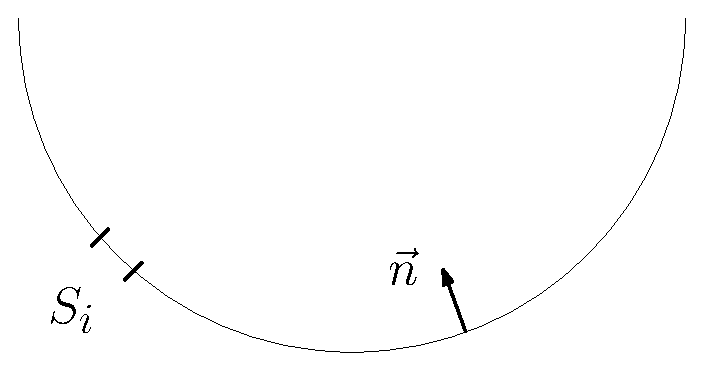
\includegraphics[width=4cm]{Si.eps}
\end{minipage}

\noindent\begin{minipage}{.45\textwidth}
Forholdene $\md x$ og $\md y$ kan enkelt vises v.h.a formlike trekanter.
\end{minipage}\hfill
\begin{minipage}{.45\textwidth}
\includegraphics[width=4.5cm]{dxdydS.eps}
\end{minipage}

\begin{align}
  \int_{S_i} \pder{}{n}\ln r\md S &= \int_{S_i} \big(\md Sn_1\pder{}{x} +
                              \md Sn_2\pder{}{y}\big) \Re\{\ln z\} \notag \\
    &= \int_{S_i} \big(-\md y\pder{}{x} +\md x\pder{}{y}\big) \Re\{\ln z\}
    \label{eq:A7}
\end{align}
De deriverte i (\ref{eq:A7}) er gitt ved
\begin{align*}
  \pder{}{x}\ln z = \pder{}{x}\ln z\pder{z}{x} = \frac{1}{z} \;,\hspace{6mm}
                    \pder{}{y}\ln z=\frac{i}{z} \;,
\end{align*}
og setter vi dette inn i (\ref{eq:A7}) får vi
\begin{align}
  \int_{S_i} \pder{}{n}\ln r\md S &= \Re \int_{S_i} \frac{-\md y + i\md x}{z} \notag\\
   &= \Re \int_{S_i} \frac{i\md x + i^2\md y }{z} \notag\\
   &= \Re \int_{S_i} \frac{i\md z}{z} \notag\\
   &= \Re \{i\ln z |_{\vec{x}_{i-\frac{1}{2}}}^{\vec{x}_{i+\frac{1}{2}}}\} \label{eq:A8}\;. 
\end{align}

\noindent\begin{minipage}{.45\textwidth}
Vi har at
\begin{align*}
  \ln z &= \ln|z| + \mathrm{arg}\,z \\
  i\ln z &= i\ln|z| - \mathrm{arg}\,z \;,
\end{align*}
og (\ref{eq:A8}) kan derfor skrives
\begin{align}\label{eq:A9}
  \Re \{i\ln z |_{\vec{x}_{i-\frac{1}{2}}}^{\vec{x}_{i+\frac{1}{2}}}\} &=
            -\mathrm{arg}\,z |_{\vec{x}_{i-\frac{1}{2}}}^{\vec{x}_{i+\frac{1}{2}}}
        = -\theta^j_i \;.
\end{align}
\end{minipage}\hfill
\begin{minipage}{.45\textwidth}
  \centering
  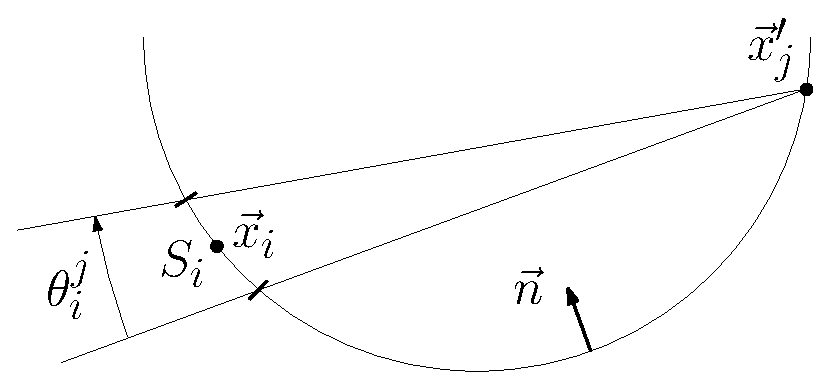
\includegraphics[width=5cm]{theta_flux.eps}
  \captionof*{figure}{Fysisk er $\theta^j_i$ gitt som fluksen ut av en åpningsvinkel.}
\end{minipage}
%%%%%%%%%%%%%%%%%%%%%%%%%%%%%%%%%%%%%%%%%%%%%%%%%%%%%%%%%%%%%%%%%%% Diskretisering
\newpage
V.h.a (\ref{eq:A9}) kan vi skrive ligningene (\ref{eq:A5a}) og (\ref{eq:A5b}) på
diskretisert form
\begin{align}\label{eq:A10a}
  \pi\Phi_j + \sum_{i=1}^{N}\Psi_i \theta_i^j = 0\;,
\end{align}
\begin{align}\label{eq:A10b}
  \pi\Psi_j + \sum_{i=1}^{N}\Phi_i \theta^j_i
     + 2\rho i\omega \frac{b}{\mu} \sum_{i=1}^{N} \Psi_i \int_{S_i}\ln r_{j,i}\md S
        &= -2u_0\sum_{i=1}^{N}n_{1,i}\int_{S_i}\ln r_{j,i} \md S \;.
\end{align}
% Vi kan sette inn for $\Phi$ inn i (\ref{10b}) og få ut en ligning bare for
% $\Psi$,
% \begin{align}\tag{11a}\label{11a}
%   \pi\Psi_j - \sum_{i=1}^{N}\left(-\frac{1}{\pi}\sum_{k=1}^N\Psi_k\theta_k^i\right)
%    \theta^j_i
%      - 2\frac{\rho i\omega b}{\mu} \sum_{i=1}^{N} \Psi_i \int_{S_i}\ln r_{j,i}\md S
%         &= 2u_0\sum_{i=1}^{N}n_{1,i}\int_{S_i}\ln r_{j,i} \md S \;.
% \end{align}
% \begin{align}\tag{11b}\label{11b}
%   \pi\Psi_j +\frac{1}{\pi} \sum_{k=1}^{N}\Psi_k\left(\sum_{i=1}^N\theta_k^i\theta^j_i
%                                                                           \right)
%      - 2\frac{\rho i\omega b}{\mu} \sum_{i=1}^{N} \Psi_i \int_{S_i}\ln r_{j,i}\md S
%         &= 2u_0\sum_{i=1}^{N}n_{1,i}\int_{S_i}\ln r_{j,i} \md S \;.
% \end{align}
% $\Phi$ finner vi ved å sette inn for $\Psi$ i (\ref{10a}) etter denne er regnet
% ut.
Til slutt finner vi $\phi_e$ og $\phi_i$ ved
\begin{align*}
  \phi_e = \frac{1}{2}(\Phi + \Psi) \;, \\
  \phi_i = \frac{1}{2}(\Phi - \Psi) \;.
\end{align*}

\subsection*{Implementering}
For å løse dette numerisk setter vi ligning (\ref{eq:A10a}) inn i (\ref{eq:A10b}),
og løser følgende matrisesystem:
\begin{align*}
  \begin{pmatrix}
    \pi & 0 & \cdots & 0 & \theta^1_1 & \theta^1_2 & \cdots & \theta^1_N \\
    0 & \pi &  & \vdots & \theta^2_1 & \theta^2_2 &  & \vdots \\
    \vdots & & \ddots & 0 & \vdots & & \ddots & & & \\
    0 & \cdots & 0 & \pi & \theta^1_N & \cdots & & \theta^N_N \\
    \theta^1_1 & \theta^2_1 & \cdots & \theta^N_1 & \pi+\alpha_1^1 & \alpha_1^2 & \cdots & \alpha^N_1 \\
    \theta^1_2 & \theta^2_2 &  & \vdots & \alpha^1_2 & \pi+\alpha^2_2 &  & \vdots \\
    \vdots & & \ddots & & \vdots & & \ddots &  \\
    \theta^1_N & \cdots & & \theta^N_N & \alpha_N^1 & \cdots &  & \pi+\alpha^N_N
  \end{pmatrix}
  \begin{pmatrix}
    \Phi_1 \\ \vdots \\ \Phi_N \\ \Psi_1 \\ \vdots \\ \Psi_N
  \end{pmatrix} = 
  \begin{pmatrix}
    0 \\ \vdots \\ 0 \\  -\beta^j_1 \\ \vdots \\ -\beta^j_N
  \end{pmatrix} \;,
\end{align*}
hvor $\alpha$ og $\beta$ er gitt ved
\begin{align*}
  \alpha^j_i &= 2\rho i\omega \frac{b}{\mu}\int_{S_i}\ln r^j_i \md S\;,\\
  \beta^j_i &= 2i\omega d\sum_{i=1}^Nn_{1,i}\int_{S_i}\ln r_i^j \md S\;.
\end{align*}

%%%%%%%%%%%%%%%%%%%%%%%%%%%%%%%%%%%%%%%%%%%%%%%%%%%%%%%%%%%%%%%%%%%%%%%%%
\end{document}
